\chapter{Methodology}
\label{methodology}

\section{Project management methodology}
I will use an iterative, evolutionary method. This will involve:
\begin{itemize}
  \item Requirements elicitation.
  \begin{itemize}
    \item This involves determening the needs of the user and defining requirements to meet those ends.
  \end{itemize}
  \item Feature design (UI).
  \begin{itemize}
    \item Features will be designed at first using wireframe models. Then on later iterations, colour and shading will be added alongside further considerations usability such as highlight on hover etc.
  \end{itemize}
  \item Feature implementation research.
  \begin{itemize}
    \item This step involves determining the apropriate technologies and libraries to achieve the design. This is nececarry to realize the constraints that are imposed by the implementation method and know to what extent the design is feasible.
  \end{itemize}
  \item Feature implementation.
  \begin{itemize}
    \item Writing the code to create the feature.
  \end{itemize}
  \item Feature testing.
  \begin{itemize}
    \item Initially testing will be done manually with valid values until later iterations whereby extraneous values will be introduced. Once the feature is in it's final iterations a unit test will be introduced.
  \end{itemize}
  \item Evaluation.
  \begin{itemize}
    \item Does the feature meet the requirements and fulfill the needs of the user?
  \end{itemize}
\end{itemize}
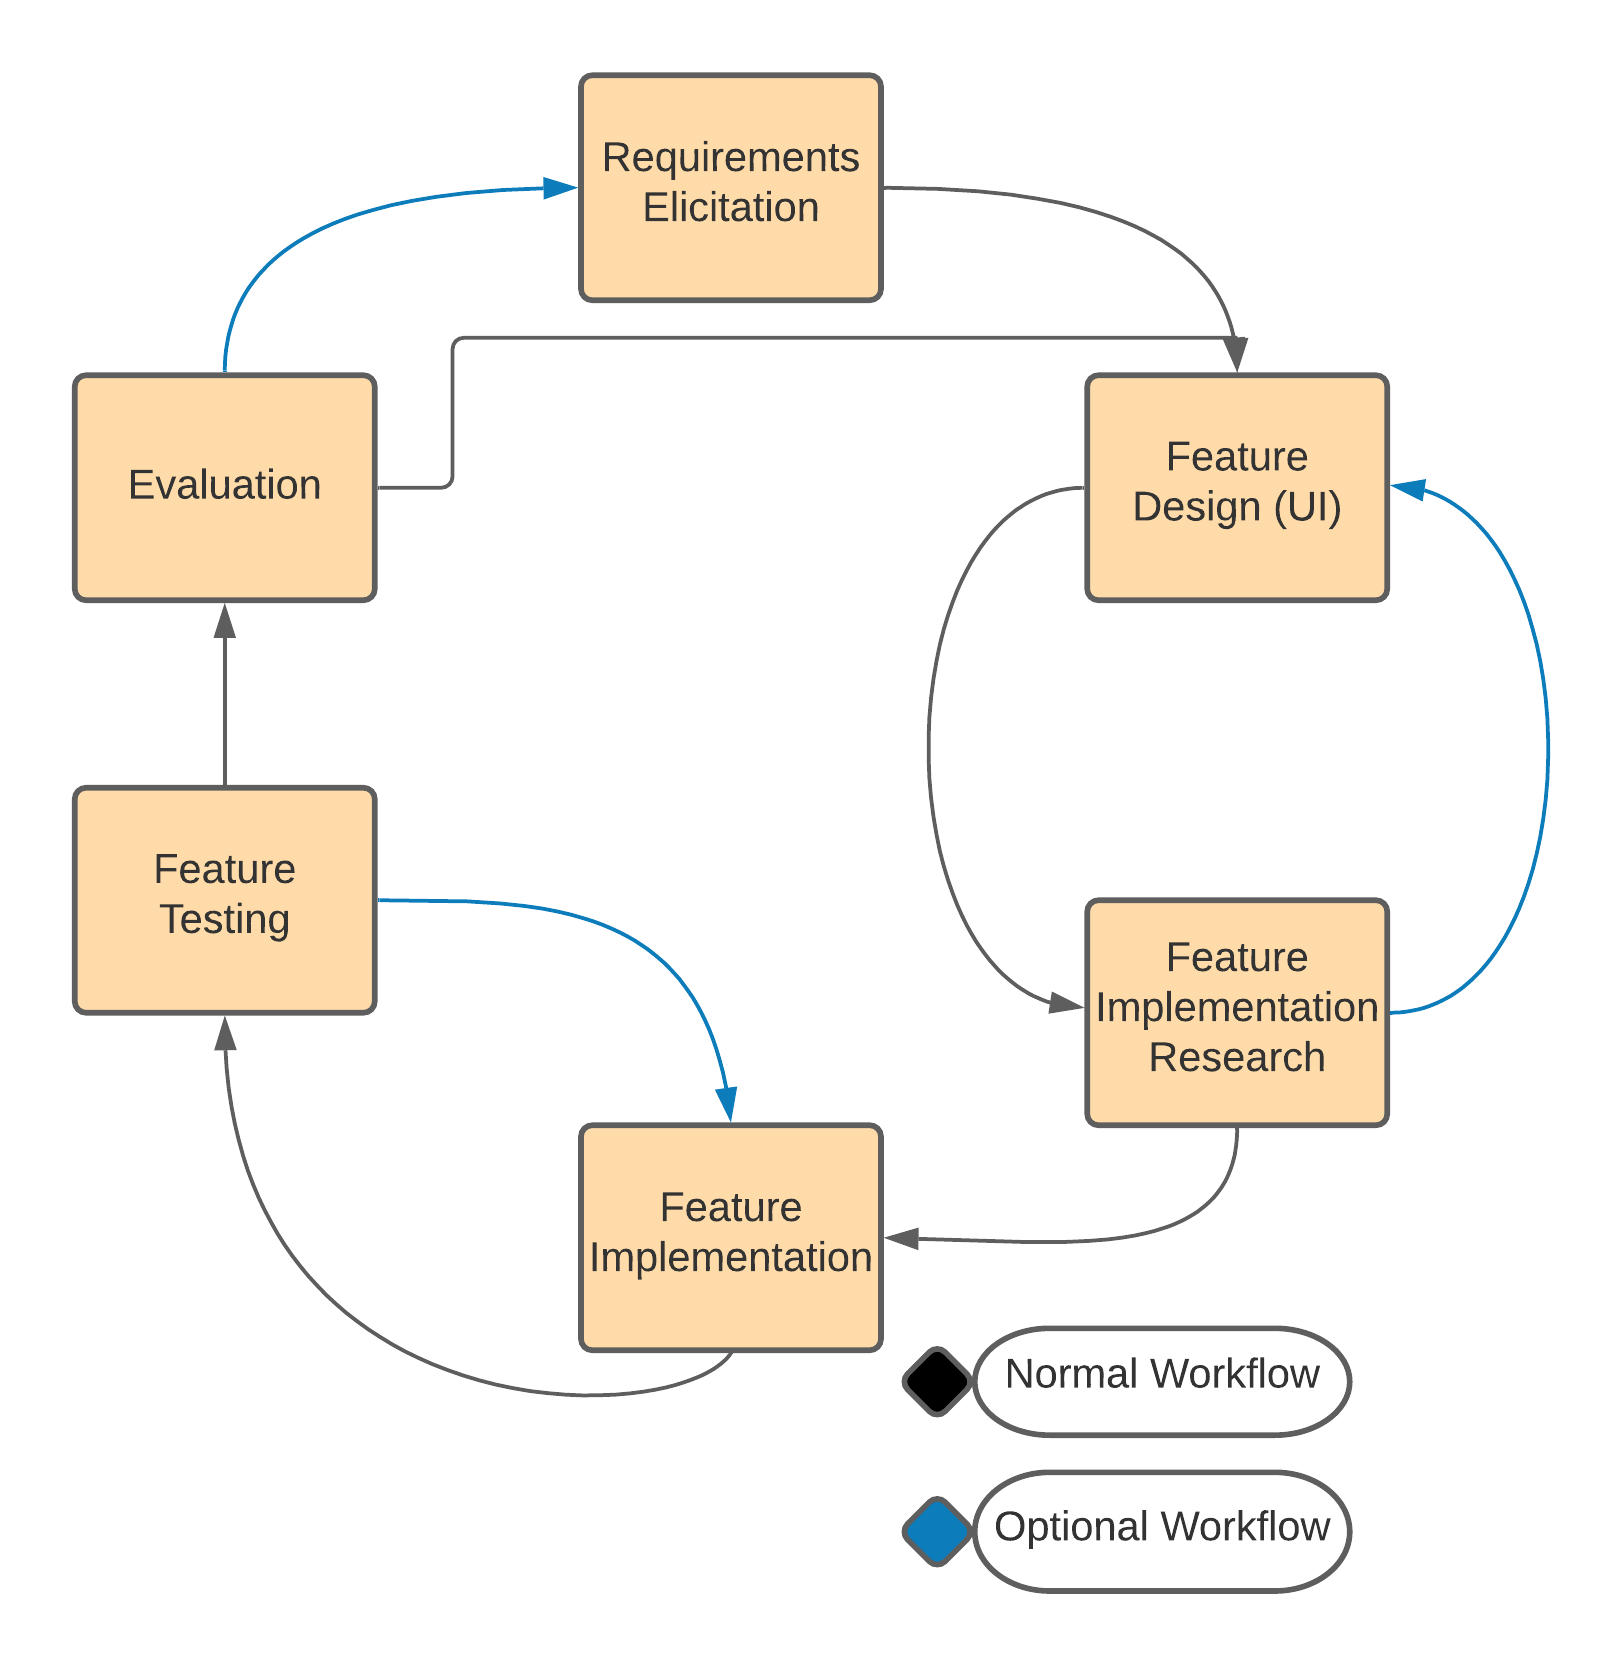
\includegraphics{Images/Project_Management_Methodology}
\section{Evaluation Design}
 (what method(s), used how, with what and how many participants?)

\section{Requirements Elicitation}
  How will requirements of the software be determined.

\section{Feature management}
  e.g., kanban boards

\section{Design Methods}
   (e.g., wireframes, DFDs, use case diagrams, class diagrams, sequence diagrams, ERDs, etc)

\section{Testing methods}

\section{Version control}
  I will be using git and github

\section{Evaluation methods}
  e.g. SUS (system usability scale)

\section{Requirements}
  TEST TEXT
\section{Desing and Implementation details}

\section{Justification of Implementation Choices}
